% SIMODS version (one idea: groups are factors); built from structure_B. Earlier header: (one idea: groups are factors; theory -> learning within -> across -> evidence).

% ---- begin ../shared/docclass.tex
% Document class selection (\input as the first line of each main.tex).
% SIMODS is typeset with SIAM's online-journal class siamonline<date>.cls. The class is not on CTAN;
% download it from SIAM's author page (the CI tries to) and place it in paper/shared/siam/.
% Without it the paper builds with a compatible fallback (article + siamshim.tex), so that text,
% numbering and cross-references can be checked; the submission must use the official class.
\makeatletter
\let\pf@cls\relax
\IfFileExists{siamonline220329.cls}{\def\pf@cls{siamonline220329}}{}
\IfFileExists{siamonline250211.cls}{\def\pf@cls{siamonline250211}}{}
\ifx\pf@cls\relax
  \documentclass[11pt]{article}
  \def\paperclass{shim}
\else
  \edef\pf@doc{\noexpand\documentclass[supplement,onefignum,onetabnum]{\pf@cls}}
  \pf@doc
  \def\paperclass{siam}
\fi
\makeatother

% ---- end ../shared/docclass.tex


% ---- begin ../shared/preamble.tex
% Common preamble of both papers (after docclass.tex).
\def\pfshimname{shim}
\ifx\paperclass\pfshimname
  
% ---- begin ../shared/siamshim.tex
% Fallback that mimics the parts of siamonline used by the papers (only when the class is absent).
\usepackage[letterpaper,margin=1.15in]{geometry}
\usepackage{amsmath,amssymb,amsthm}
\usepackage[T1]{fontenc}
\usepackage{lmodern}
\usepackage{fancyhdr}
\newcommand{\headers}[2]{\pagestyle{fancy}\fancyhf{}\fancyhead[LE]{\small\thepage\quad\textsc{#2}}%
  \fancyhead[RO]{\small\textsc{#1}\quad\thepage}\fancyhead[LO,RE]{}\renewcommand{\headrulewidth}{0pt}}
\newcommand{\email}[1]{\texttt{#1}}
\newcommand{\funding}[1]{\par\noindent\textbf{Funding:} #1}
\newenvironment{keywords}{\par\smallskip\noindent\textbf{Key words.}\ }{\par}
\newenvironment{MSCcodes}{\par\smallskip\noindent\textbf{MSC codes.}\ }{\par}
\newenvironment{AMS}{\par\smallskip\noindent\textbf{AMS subject classifications.}\ }{\par}
\renewenvironment{abstract}{\par\small\noindent\textbf{Abstract.}\ }{\par\normalsize}

% ---- end ../shared/siamshim.tex

\else
  \usepackage{amssymb}
  \newsiamremark{remark}{Remark}
  \newsiamremark{example}{Example}
  \newsiamthm{assumption}{Assumption}
\fi
\usepackage{mathtools}
\usepackage{graphicx}
\graphicspath{{figures/simods/}{figures/}}
\usepackage{booktabs,array,tabularx,multirow}
\usepackage[dvipsnames]{xcolor}
\usepackage{tikz}
\usetikzlibrary{arrows.meta,positioning,calc,fit,shapes.geometric,backgrounds}
\usepackage{algorithm}
\usepackage{algpseudocode}
\usepackage{enumitem}
\setlist{nosep,leftmargin=*}
\ifx\paperclass\pfshimname
  \usepackage[hidelinks]{hyperref}
  \usepackage[capitalize,nameinlink]{cleveref}
  
% ---- begin ../shared/siamshim_thm.tex
% Fallback theorem environments (loaded after hyperref and cleveref so that names resolve).
\theoremstyle{plain}
\newtheorem{theorem}{Theorem}[section]
\newtheorem{lemma}[theorem]{Lemma}
\newtheorem{proposition}[theorem]{Proposition}
\newtheorem{corollary}[theorem]{Corollary}
\theoremstyle{definition}
\newtheorem{definition}[theorem]{Definition}
\newtheorem{assumption}[theorem]{Assumption}
\theoremstyle{remark}
\newtheorem{remark}[theorem]{Remark}
\newtheorem{example}[theorem]{Example}

% ---- end ../shared/siamshim_thm.tex

\else
  \makeatletter\@ifpackageloaded{cleveref}{}{\usepackage[capitalize,nameinlink]{cleveref}}\makeatother
\fi
\crefname{assumption}{Assumption}{Assumptions}
\crefname{example}{Example}{Examples}
\crefname{remark}{Remark}{Remarks}
\crefname{algorithm}{Algorithm}{Algorithms}

% ---- begin ../shared/macros.tex
% ---------------------------------------------------------------------------------------------
% Notation macros. ONE symbol, ONE meaning: every macro below is listed in the notation table
% (sections/notation.tex) and the script tools/check_notation.py checks the correspondence.
% ---------------------------------------------------------------------------------------------
% number sets and rings
\newcommand{\R}{\mathbb{R}}
\newcommand{\C}{\mathbb{C}}
\newcommand{\Z}{\mathbb{Z}}
\newcommand{\ring}{\mathcal{R}}            % ring of constant-coefficient operators C[d_t,d_x] = C[tau,xi]
% operators and their algebra
\DeclareMathOperator{\Ann}{Ann}             % annihilator ideal of a function
\DeclareMathOperator{\gcdop}{gcd}
\DeclareMathOperator{\spn}{span}
\DeclareMathOperator{\rank}{rank}
\DeclareMathOperator{\diag}{diag}
\DeclareMathOperator{\tr}{tr}
\newcommand{\Var}{V}                        % characteristic variety V(P)
\newcommand{\EP}{\mathrm{EP}}               % exponential-polynomials
\newcommand{\dd}{\,\mathrm{d}}
\newcommand{\Id}{\mathrm{Id}}
\newcommand{\Gu}{G_u}                       % intrinsic operator gcd Ann(u)
\newcommand{\Ju}{J_u}                       % cofactor ideal, Ann(u) = G_u J_u
\newcommand{\sigp}{\Sigma_{\mathrm p}}      % point spectrum V(J_u)
\newcommand{\sumop}{\mathcal{S}}            % sum operator (u_1,...,u_N) -> sum u_j
\newcommand{\Eint}{E_{\mathrm{int}}}        % interaction term
\newcommand{\flow}{\Phi}                    % flows Phi_n(t) = e^{t A_n}
\newcommand{\cF}{c_{F}}                     % Friedrichs cosine
\newcommand{\thetaF}{\theta_{F}}            % Friedrichs angle
\newcommand{\gN}{\gamma_{N}}                % conditioning constant of the sum operator
\newcommand{\deltaP}{\delta(P)}             % ambiguity dimension
\newcommand{\Hs}{H^{s}}                     % Sobolev space of index s
\newcommand{\noise}{\sigma_{n}}             % observation noise standard deviation
\newcommand{\sigbin}{\sigma_{\kappa}}       % noise standard deviation of one Fourier bin
\newcommand{\Nsamp}{N_{\mathrm s}}          % number of posterior field samples
\newcommand{\keff}{k_{\mathrm{eff}}}        % effective number of factors
\newcommand{\cloud}{W}                      % cloud of factor vectors (a weighted point measure)
\newcommand{\Mfit}{\mathsf{M}}              % a candidate structure (model)
\newcommand{\lab}[1]{\textsf{#1}}           % output labels
\newcommand{\FC}{\lab{FIT-COMPATIBLE}}
\newcommand{\IDK}{\lab{ID-KER}}
\newcommand{\MIS}{\lab{MISFIT}}
\newcommand{\UND}{\lab{UNDECIDED}}
\newcommand{\Normal}{\mathcal{N}}
\newcommand{\E}{\mathbb{E}}
\newcommand{\abs}[1]{\lvert#1\rvert}
\newcommand{\norm}[1]{\lVert#1\rVert}
\newcommand{\ip}[2]{\langle#1,#2\rangle}
% editorial
\newcommand{\roleinalg}[1]{\par\noindent\emph{Role in the algorithm.} #1\par}
\newcommand{\inbrief}[1]{\par\smallskip\noindent\emph{In brief.} #1\par\smallskip}

% ---- end ../shared/macros.tex


% ---- end ../shared/preamble.tex



% ---- typography
\usepackage[T1]{fontenc}
\usepackage{lmodern}
\usepackage[final]{microtype}
\renewcommand{\topfraction}{0.9}
\renewcommand{\bottomfraction}{0.8}
\renewcommand{\textfraction}{0.07}
\renewcommand{\floatpagefraction}{0.85}
\setcounter{topnumber}{3}
\setcounter{bottomnumber}{2}
\setcounter{totalnumber}{4}
\setlength{\abovecaptionskip}{6pt}
\usepackage{needspace}
\makeatletter\ifx\paperclass\pfshimname\else\externaldocument[][nocite]{simods}\fi\makeatother

\title{Groups Are Factors: Learning Linear PDEs\\by Clustering Modes on the Factors of the Symbol}
\author{Flavio Pricoco\thanks{\email{flaflapr@gmail.com}}}
\headers{Groups are factors: learning linear PDEs}{F. Pricoco}

\begin{document}
\maketitle

\noindent These supplementary materials accompany the paper and are not needed to follow it. They contain the notation
(\cref{sm:notation}); the proofs of the main results, written to be read rather than only checked
(\cref{sm:proofs}); the interaction of terms inside a factor (\cref{sm:interaction}); the complete algorithm and its
parameters (\cref{sm:algo}); further cases and a guide to reading the output (\cref{sm:cases}); what carries over
beyond linear equations with constant coefficients (\cref{sm:beyond}); and the contents of the code and data archive
(\cref{sm:code}). Numbers without the prefix SM refer to the paper.

\section{Notation}\label{sm:notation}
\begin{table}[htbp]
\centering\small
\caption{Notation. Each symbol has one meaning in the paper and in these materials.}\label{sm:tab:notation}
\begin{tabularx}{\linewidth}{@{}l >{\raggedright\arraybackslash}X@{}}
\toprule
Symbol & Meaning\\
\midrule
$\ring=\C[\tau,\xi]$ & constant-coefficient operators; $\tau\leftrightarrow\partial_t$, $\xi\leftrightarrow\partial_x$\\
$P,\ Q_j,\ P_i,\ e_i$ & an operator and its symbol; a factor; an irreducible factor and its multiplicity\\
$\Var(P)$ & characteristic variety, the zero set of $P$ in $\C^2$\\
$\kappa,\ \lambda(\kappa)$ & real wavenumber ($\xi=i\kappa$); temporal rate of the mode $e^{\lambda t+i\kappa x}$\\
$\Lambda_j(\xi)$ & branch of an evolution factor $Q_j=\tau-\Lambda_j(\xi)$\\
$\Ann(u)$ & annihilator: all operators $Q$ with $Q(\partial)u=0$\\
$\EP$ & exponential-polynomials, finite sums $\sum p_j(t,x)e^{\tau_jt+\xi_jx}$\\
$N,\ \deltaP$ & number of factors; dimension of the overlap of their solution spaces\\
$\sumop,\ \gN$ & sum operator $(u_1,\dots,u_N)\mapsto\sum_ju_j$; its conditioning constant\\
$\cF,\ \thetaF$ & Friedrichs cosine and angle; for two factors $\gamma_2=1-\cF$\\
$\Eint,\ \rho$ & interaction term; interaction ratio $\norm{\Eint}/\norm{u(T)-u_0}$\\
$w_j$ & energy share of group $j$\\
$\noise,\ \sigbin$ & noise standard deviation; its value in one Fourier bin\\
$\mathcal K,\ z$ & band of usable wavenumbers; detection threshold in units of $\sigbin$\\
$A_p,\ \sigma_{\lambda,p}$ & amplitude of mode $p$; standard deviation of its rate\\
$\Nsamp,\ u^{(q)},\ \pi_q$ & number of posterior field samples; sample $q$; its weight\\
$\Mfit$; $C(m,d)$ & a structure (number and degrees of the factors); a class of structures\\
$B_j$; $\omega^2$ & orthonormal basis of the sampled kernel of $Q_j$; prior variance of the component coefficients\\
$\cloud$; $\alpha$; $k$ & cloud of factor vectors; Dirichlet-process concentration; number of groups\\
\FC, \IDK, \MIS, \UND & output labels\\
\bottomrule
\end{tabularx}
\end{table}

\section{Proofs of the main results}\label{sm:proofs}
We prove in full the results the algorithm rests on: the factor decomposition (\cref{thm:factor}), the stability of the
split (\cref{thm:hm}), its Bayesian form (\cref{prop:bayes-angle}) and the counting condition (\cref{prop:counting}).
For identification and finite data (\cref{thm:ident,prop:certify}) we give the idea and an example, and prove the part
that matters for the algorithm. Complete proofs of every statement, in a longer form, are in the analytical notes of the
repository~\cite{Pri26code}.

Throughout, $\Omega\subset\R^2$ is open and connected, $\mathcal A$ is $C^\infty(\Omega)$ or the distributions
$\mathcal D'(\Omega)$, and a polynomial $Q\in\ring$ acts on $\mathcal A$ by $\tau\mapsto\partial_t$, $\xi\mapsto\partial_x$.
For a point $z=(\tau_z,\xi_z)\in\C^2$ we write $\psi_z(t,x)=e^{\tau_zt+\xi_zx}$.

\subsection{Four facts from algebra}\label{sm:algebra}
The proofs use four classical facts about polynomials in two variables~\cite{CLO15,Ful08}. We state them in the form
used and say why each is true.
\begin{enumerate}[label=(F\arabic*), leftmargin=*]
\item \emph{Unique factorization.} Every polynomial is a product of irreducible ones, uniquely up to order and constants.
Consequently, if $Q_1$ and $Q_2$ have no common factor, a polynomial divisible by both is divisible by $Q_1Q_2$:
$(Q_1)\cap(Q_2)=(Q_1Q_2)$.
\item \emph{Coprime curves meet in finitely many points.} If $Q_1,Q_2$ have no common factor, $\Var(Q_1)\cap\Var(Q_2)$ is
finite. (Viewed as polynomials in $\tau$ with coefficients rational in $\xi$, they have a B\'ezout identity
$aQ_1+bQ_2=r(\xi)$ with a nonzero polynomial $r$; at a common zero $r(\xi)=0$, which leaves finitely many $\xi$, and
symmetrically finitely many $\tau$.)
\item \emph{Finitely many common zeros means finite codimension.} If an ideal $I$ has a finite zero set, the quotient
$\ring/I$ is a finite-dimensional vector space (Hilbert's Nullstellensatz). In particular $\dim\ring/(Q_1,Q_2)<\infty$
for coprime $Q_1,Q_2$.
\item \emph{Intersection numbers add.} For coprime $Q_1,Q_2$, $\dim\ring/(Q_1,Q_2)$ is the number of intersection points of
the two curves counted with multiplicity, and the multiplicities are additive: the intersection of $Q_1$ with $Q_2Q_3$
is the intersection with $Q_2$ plus the intersection with $Q_3$~\cite[Ch.~3]{Ful08}.
\end{enumerate}

\subsection{Exponential-polynomials}\label{sm:ep}
One more fact is about functions: an exponential-polynomial is exactly a function whose derivatives span a
finite-dimensional space.
\begin{lemma}[Finite-dimension criterion]\label{sm:lem:ep}
A function or distribution $w$ on a connected $\Omega$ is an exponential-polynomial if and only if the span $R_w$ of all
its derivatives $\partial_t^j\partial_x^kw$ is finite-dimensional. Its exponents are then the joint eigenvalues of
$\partial_t$ and $\partial_x$ on $R_w$.
\end{lemma}
\begin{proof}[Idea of the proof]
If $w=p(t,x)e^{at+bx}$, then $\partial_tw=(p_t+ap)e^{at+bx}$ and $\partial_xw=(p_x+bp)e^{at+bx}$: differentiation never
raises the degree of $p$, so all derivatives stay in the finite-dimensional space of (polynomials of degree at most
$\deg p$)$\,\times e^{at+bx}$. Conversely, if $R_w$ is finite-dimensional, $\partial_t$ and $\partial_x$ act on it as two
commuting matrices; their minimal polynomials $m_t,m_x$ give two ordinary differential equations $m_t(\partial_t)w=0$
and $m_x(\partial_x)w=0$, whose common solutions on a rectangle are exponential-polynomials, and connectedness extends
this to $\Omega$.
\end{proof}
The matrix pencil of \cref{sec:modes} is exactly this eigenvalue computation for $\partial_t$, one wavenumber at a time.

\subsection{The factor decomposition}\label{sm:proof-factor}
\paragraph{What has to be shown} For two coprime factors $Q_1,Q_2$ consider the sum map
\[
  \Sigma:\ \ker Q_1\oplus\ker Q_2\to\ker(Q_1Q_2),\qquad (u_1,u_2)\mapsto u_1+u_2 .
\]
It is well defined, because $Q_1Q_2(u_1+u_2)=Q_2(Q_1u_1)+Q_1(Q_2u_2)=0$. \Cref{thm:factor} for two factors says two
things: $\Sigma$ is \emph{onto} (every solution splits), and its kernel has dimension $\dim\ring/(Q_1,Q_2)$ (the
ambiguity is the number of intersection points). The kernel is easy: $\Sigma(u_1,u_2)=0$ means $u_2=-u_1$ with $u_1$
killed by both factors, so
\[
  \ker\Sigma=\{(v,-v):\ Q_1v=Q_2v=0\}.
\]
The common solutions of $Q_1$ and $Q_2$ are killed by the whole ideal $(Q_1,Q_2)$, whose zero set is finite (F2), so by
\cref{sm:lem:ep} they are exponential-polynomials, one exponential for each common zero (times polynomials at a zero of
higher multiplicity). The hard part is that $\Sigma$ is onto.

\paragraph{The one-variable case, and what goes wrong in two} In one variable two coprime polynomials satisfy B\'ezout's
identity $aQ_1+bQ_2=1$, and then $u=b(\partial)Q_2(\partial)u+a(\partial)Q_1(\partial)u$ is the split: the first piece is
killed by $Q_1$ because $Q_1bQ_2u=b\,Q_1Q_2u=0$, the second by $Q_2$. In two variables coprime polynomials need not
generate $1$: $\tau+c\xi$ and $\tau-\nu\xi^2$ both vanish at $(0,0)$, so every combination of them vanishes there too.
The quotient $\ring/(Q_1,Q_2)$, finite-dimensional by (F3), measures exactly how far we are from B\'ezout. The proof shows
that this defect costs nothing for solvability, only the finite ambiguity, provided the domain has no holes.

\paragraph{Step 1: one point, one potential} Fix a point $z$ and ask: given $a,b\in\mathcal A$ with
\begin{equation}\label{sm:eq:compat}
  (\partial_t-\tau_z)\,b=(\partial_x-\xi_z)\,a ,
\end{equation}
is there a $v\in\mathcal A$ with $(\partial_t-\tau_z)v=a$ and $(\partial_x-\xi_z)v=b$? Condition \eqref{sm:eq:compat} is
clearly necessary, since the two operators commute. Write $a=\psi_z\tilde a$, $b=\psi_z\tilde b$, $v=\psi_z\tilde v$; because
$(\partial_t-\tau_z)(\psi_z\tilde v)=\psi_z\,\partial_t\tilde v$, the question becomes: given a vector field
$(\tilde a,\tilde b)$ with $\partial_t\tilde b=\partial_x\tilde a$ (no curl), is it a gradient,
$(\tilde a,\tilde b)=(\partial_t\tilde v,\partial_x\tilde v)$? On a simply connected domain the answer is yes, for smooth
fields by the Poincar\'e lemma and for distributions by de Rham's theorem~\cite{Rha55}. In the language of homological
algebra: $\operatorname{Ext}^1_\ring(\ring/\mathfrak m_z,\mathcal A)=H^1_{\mathrm{dR}}(\Omega)=0$, where $\mathfrak m_z$ is
the ideal of polynomials vanishing at $z$. The solutions of the homogeneous problem, $a=b=0$, are the multiples of
$\psi_z$, a space of dimension one.

\paragraph{Step 2: finitely many points} Let $M$ be any $\ring$-module of finite dimension over $\C$, for instance
$M=\ring/(Q_1,Q_2)$. Such a module is built from one-point modules $\ring/\mathfrak m_z$ by finitely many extensions
(a composition series). For each extension $0\to M'\to M\to M''\to0$ the long exact sequence of
$\operatorname{Hom}(\cdot,\mathcal A)$ shows that if the solvability problem of Step~1 has no obstruction for $M'$ and
$M''$, it has none for $M$, and that the dimensions of the solution spaces add. By induction on $\dim M$,
\begin{equation}\label{sm:eq:ext}
  \operatorname{Ext}^1_\ring(M,\mathcal A)=0,\qquad \dim\operatorname{Hom}_\ring(M,\mathcal A)=\dim_\C M .
\end{equation}
Here $\operatorname{Hom}_\ring(\ring/I,\mathcal A)$ is simply the space of solutions of all equations in $I$: a module
homomorphism is determined by the image $v$ of $1$, and it is well defined exactly when $Q(\partial)v=0$ for all $Q\in I$.

\paragraph{Step 3: two factors} By (F1) the sequence
\[
  0\to\ring/(Q_1Q_2)\xrightarrow{\ r\mapsto(r,r)\ }\ring/(Q_1)\oplus\ring/(Q_2)\xrightarrow{\ (r,s)\mapsto r-s\ }\ring/(Q_1,Q_2)\to0
\]
is exact: the first map is injective because $(Q_1)\cap(Q_2)=(Q_1Q_2)$, and the kernel of the second consists of pairs
$(r,s)$ with $r-s=xQ_1+yQ_2$, which are the image of $r-xQ_1=s+yQ_2$. Applying $\operatorname{Hom}_\ring(\cdot,\mathcal A)$
turns each quotient $\ring/I$ into the solutions of $I$ and gives the exact sequence
\[
  0\to\ker Q_1\cap\ker Q_2\xrightarrow{\ v\mapsto(v,-v)\ }\ker Q_1\oplus\ker Q_2\xrightarrow{\ \Sigma\ }\ker(Q_1Q_2)\to
  \operatorname{Ext}^1_\ring\big(\ring/(Q_1,Q_2),\mathcal A\big).
\]
The last group vanishes by \eqref{sm:eq:ext}, because $\ring/(Q_1,Q_2)$ is finite-dimensional (F3). So $\Sigma$ is onto,
and its kernel, the common solutions, has dimension $\dim\ring/(Q_1,Q_2)$, again by \eqref{sm:eq:ext}.

\paragraph{Step 4: more factors} Let $P=Q_1\cdots Q_N$ with pairwise coprime $Q_j$, and $P'=Q_2\cdots Q_N$. Then $Q_1$ and
$P'$ are coprime (F1), so by Step~3 $\ker P=\ker Q_1+\ker P'$, and by induction $\ker P'=\sum_{j\ge2}\ker Q_j$. This gives
the decomposition~\eqref{eq:split}. The full sum map $\bigoplus_j\ker Q_j\to\ker P$ is the composition of
$\bigoplus_{j\ge2}\ker Q_j\to\ker P'$ (kernel of dimension $\delta(P')$ by induction) and of
$\ker Q_1\oplus\ker P'\to\ker P$ (kernel of dimension $\dim\ring/(Q_1,P')$ by Step~3); both are onto, so the kernel
dimensions add, and by (F4) $\dim\ring/(Q_1,P')=\sum_{j\ge2}\dim\ring/(Q_1,Q_j)$. This is formula~\eqref{eq:delta}.
\hfill$\square$

\begin{example}[Running example]\label{sm:ex:delta}
For $Q_1=\tau+c\xi$ and $Q_2=\tau-\nu\xi^2$, substitute $\tau=-c\xi$ into $Q_2$: $-c\xi-\nu\xi^2=-\xi(c+\nu\xi)$, with the two
simple roots $\xi=0$ and $\xi=-c/\nu$. So the curves meet at $(0,0)$ and $(c^2/\nu,-c/\nu)$, each once, and
$\deltaP=\dim\ring/(Q_1,Q_2)=2$. The ambiguous pairs are $(v,-v)$ with $v$ a combination of $1$ and
$e^{(c^2/\nu)t-(c/\nu)x}$: exactly the functions that can be moved between the transport and the diffusion group.
\end{example}

\paragraph{Why the domain matters} Only Step~1 uses the shape of $\Omega$, and it fails on a domain with a hole: on an
annulus the field $(\tilde a,\tilde b)=\nabla\arg z$ has no curl but is not a gradient. This is the obstruction behind the
example of the Laplacian in \cref{sec:factor}.

\subsection{Stability of the split}\label{sm:proof-hm}
\begin{proof}[Proof of \cref{thm:hm}]
The sum operator $\sumop:\bigoplus_jM_j\to\ker_{\Hs}P$ is bounded, by the triangle and Cauchy--Schwarz inequalities,
$\norm{\sum_ju_j}^2\le N\sum_j\norm{u_j}^2$. Every $u$ in its range has components in $\Hs$ by definition, so ``every
$u\in\ker_{\Hs}P$ has components in $\Hs$'' means that the range is all of $\ker_{\Hs}P$, i.e.\ that it is closed and
dense. By the closed range theorem~\cite[Thm.~2.21]{Bre11}, the range is closed if and only if $\sumop$ is bounded below on
the orthogonal complement of its kernel, which is the statement $\gN>0$ by the definition~\eqref{eq:gammaN}. In that
case take, for a given $u$, the preimage $v=(u_1,\dots,u_N)$ orthogonal to $\ker\sumop$, which is the one of minimum norm;
then $\norm{u}^2=\norm{\sumop v}^2\ge\gN\norm{v}^2$, which is~\eqref{eq:hm}. In finite dimension every linear map has
closed range, and the range is the span of the sampled exponentials of $P$, each of which lies in the kernel of one
factor.
\end{proof}

\paragraph{The two-factor case, in a picture} Why is $\gamma_2=1-\cF$? Take unit vectors $u_1\in M_1$ and $u_2\in M_2$.
Then $\norm{u_1-u_2}^2=2-2\operatorname{Re}\ip{u_1}{u_2}$, while the pair has norm $\sqrt2$, so the ratio in
\eqref{eq:gammaN} is $1-\operatorname{Re}\ip{u_1}{u_2}$. It is smallest when $u_1$ and $u_2$ are as aligned as possible,
i.e.\ when $\operatorname{Re}\ip{u_1}{u_2}=\cos\thetaF$, after excluding the directions the two spaces share, which form
$\ker\sumop$. \Cref{sm:proof-bayes} makes this exact through the principal angles; for infinite-dimensional spaces
see~\cite[Ch.~9]{Deu01}.

\subsection{The angle sets the error bars}\label{sm:proof-bayes}
\begin{proof}[Proof of \cref{prop:bayes-angle}]
With orthonormal bases $B_1,B_2$ of the two sampled kernels,
\[
  \sumop^H\sumop=\begin{pmatrix}I&B_1^HB_2\\ B_2^HB_1&I\end{pmatrix}.
\]
Take the singular value decomposition $B_1^HB_2=U\,\diag(\cos\theta_k)\,V^H$; the singular values are the cosines of the
principal angles $\theta_k$ between the two kernels. In the basis given by the columns of $U$ and $V$ the matrix splits into
$2\times2$ blocks $\left(\begin{smallmatrix}1&\cos\theta_k\\ \cos\theta_k&1\end{smallmatrix}\right)$, with eigenvalues
$1\pm\cos\theta_k$, plus the eigenvalue $1$ on directions of the larger kernel without a partner. The posterior covariance
$\Gamma_a=\noise^2(\sumop^H\sumop+(\noise^2/\omega^2)I)^{-1}$ is diagonal in the same basis, with variance
$\noise^2/(\mu+\noise^2/\omega^2)$ along an eigenvector of eigenvalue $\mu$. The eigenvalue $0$ occurs exactly for
$\theta_k=0$, the directions shared by the two kernels, i.e.\ $\ker\sumop$; the smallest nonzero eigenvalue is
$1-\cos\theta_{\min}=1-\cF$, which gives~\eqref{eq:bayes-angle}. On a shared direction $\mu=0$, the variance is $\omega^2$,
the prior; the likelihood depends only on the sum $a_1+a_2$ there, so the posterior of the difference is the prior,
centred at zero, and the posterior mean splits the shared part equally.
\end{proof}
Since $1-\cos\theta=2\sin^2(\theta/2)$, the posterior standard deviation in the worst direction is about
$\noise/(\sqrt2\sin(\thetaF/2))$ while it is above the prior floor: halving a small angle doubles the error bars.

\subsection{The counting condition}\label{sm:proof-counting}
\begin{proof}[Proof of \cref{prop:counting}]
Write $\Lambda(\xi)=\sum_{k=0}^d\beta_k\xi^k$. The rates at the nodes $i\kappa_\ell$ are
$\lambda_\ell=\sum_k\beta_k(i\kappa_\ell)^k$, a linear system $V\beta=\lambda$ with the Vandermonde matrix
$V_{\ell k}=(i\kappa_\ell)^k$. With $d+1$ distinct nodes $V$ is square and invertible, so the coefficients are determined, and
$\norm{\delta\beta}\le\norm{V^{-1}}\,\norm{\delta\lambda}$. With only $d$ nodes, the polynomial
$\prod_\ell(\xi-i\kappa_\ell)$ of degree $d$ vanishes at all of them and can be added to $\Lambda$ without changing any
observed rate. When the nodes lie within a spread $h_\kappa$, the Lagrange basis polynomials that make up $V^{-1}$ have
coefficients of size $h_\kappa^{-d}$~\cite{Gau62}. For real coefficients
$\operatorname{Re}\Lambda(i\kappa)=\sum_k(-1)^k\beta_{2k}\kappa^{2k}$ and
$\operatorname{Im}\Lambda(i\kappa)=\sum_k(-1)^k\beta_{2k+1}\kappa^{2k+1}$ separate the even and the odd coefficients into
two polynomials in $\kappa^2$, with $\lfloor d/2\rfloor+1$ and $\lceil d/2\rceil$ unknowns, which is the real count.
\end{proof}

\subsection{Identification and finite data: the ideas}\label{sm:ident}
\paragraph{Identification (\cref{thm:ident})} The theorem asks when a solution $u$ of $P(\partial)u=0$ satisfies no
equation except the multiples of $P$. The idea is to remove one irreducible factor $P_i$ and look at what is left,
$v_i=(P/P_i)(\partial)u$, which solves $P_i(\partial)v_i=0$.
\begin{itemize}
\item If $v_i$ is an exponential-polynomial, it sits on finitely many points of the curve $\Var(P_i)$, and some polynomial
$h$ that is \emph{not} a multiple of $P_i$ also vanishes at those points and kills $v_i$. Then $h\cdot P/P_i$ kills $u$ but
is not a multiple of $P$: $u$ satisfies an equation that $P$ does not explain.
\item If no $v_i$ is an exponential-polynomial, each factor is ``filled'' by $u$ along a whole curve, and only multiples of
$P$ can vanish on all of these curves.
\end{itemize}
\emph{Example.} For the heat operator $P=\tau-\nu\xi^2$ there is only one factor and $v=u$. A single mode
$u=e^{-\nu\kappa^2t+i\kappa x}$ is an exponential-polynomial, and indeed it also solves the pure decay
$(\partial_t+\nu\kappa^2)u=0$, which is not a multiple of the heat operator: one mode cannot tell the heat equation from
any other equation whose curve passes through the point $(-\nu\kappa^2,i\kappa)$. The heat kernel
$t^{-1/2}e^{-x^2/(4\nu t)}$ is not an exponential-polynomial (its $x$-derivatives are polynomials of growing degree times
the same Gaussian), and every constant-coefficient equation it satisfies is a multiple of $\partial_t-\nu\partial_x^2$.
The complete proof follows the two bullets, using (F2), (F3) and \cref{sm:lem:ep}.

\paragraph{Finite data (\cref{prop:certify})} Part (ii) is the one that shapes the algorithm, and its proof is two lines.
\begin{proof}[Proof of \cref{prop:certify}(ii)]
The Taylor polynomial of order $M$ at $z_0$ has the same derivatives up to order $M$ as $u$, and polynomial interpolation
in two variables matches any finite set of sample values. Both are polynomials, hence exponential-polynomials. By
\cref{thm:ident} an exponential-polynomial never has $\Ann=(P)$ when $P$ has an irreducible factor, because removing that
factor leaves an exponential-polynomial again. So the finite data are equally consistent with a function that does not
determine $P$.
\end{proof}
Part (i) is the positive counterpart: if the derivatives of $u$ span a space of dimension at most $n$, then $u$ is an
exponential-polynomial with at most $n$ terms (counted with polynomial degree), and its derivatives of order up to $2n-1$
at one point determine its annihilator; the reason is the same as for a linear recurrence of order $n$, which is fixed by
$2n$ consecutive values. Data never supply such a bound, which is why the algorithm reports compatibility, not
identification.

\section{The interaction of terms inside a factor}\label{sm:interaction}
A factor can have several additive terms: $\tau+c\xi-\nu\xi^2$ (advection--diffusion) has two. \Cref{prop:terms} says
that such a factor cannot be split into one solution per term; this section measures what is left over.

Consider an evolution $u_t=\mathcal Au$ with $\mathcal A=\mathcal A_1+\dots+\mathcal A_K$ (the terms), its flow
$\flow(t)=e^{t\mathcal A}$ and the flows $\flow_n(t)=e^{t\mathcal A_n}$ of the single terms. If term $n$ acted alone, it
would change the initial datum by $\Delta_nu_0=(\flow_n(t)-\Id)u_0$. The \emph{interaction term} is what the true
evolution does beyond the sum of these single-term changes:
\begin{equation}\label{sm:eq:eint}
  \Eint(t)=u(t)-u_0-\sum_{n=1}^K\big(\flow_n(t)u_0-u_0\big).
\end{equation}
\begin{proposition}[Interaction term]\label{sm:prop:eint}
If the terms commute (in particular for constant coefficients),
\[
  \Eint(t)=\Big[\prod_{n=1}^K(\Id+\Delta_n)-\Id-\sum_{n=1}^K\Delta_n\Big]u_0=\sum_{|E|\ge2}\Big(\prod_{n\in E}\Delta_n\Big)u_0 ,
\]
the sum running over the subsets $E\subseteq\{1,\dots,K\}$ with at least two elements. For two terms,
$\Eint=\Delta_1\Delta_2u_0$.
\end{proposition}
\begin{proof}
Commuting terms give $\flow=\prod_n\flow_n=\prod_n(\Id+\Delta_n)$. Expanding the product over subsets and removing the
empty set and the singletons gives the formula.
\end{proof}
On a Fourier mode every term is multiplication by its symbol $\hat{\mathcal A}_n(\kappa)$, so
\[
  \widehat{\Eint}(t,\kappa)=\Big[\prod_ne^{t\hat{\mathcal A}_n(\kappa)}-1-\sum_n\big(e^{t\hat{\mathcal A}_n(\kappa)}-1\big)\Big]\hat u_0(\kappa),
\]
which costs $O(K)$ operations per wavenumber, although writing out all cross terms would need $2^K-K-1$ of them.

\emph{Example (advection--diffusion).} With the terms $-c\partial_x$ and $\nu\partial_x^2$,
$\abs{\widehat{\Eint}}/\abs{\hat u_0}=\abs{(e^{-ic\kappa t}-1)(e^{-\nu\kappa^2t}-1)}\le2$: the interaction is as large as the
solution, not a small correction. On the benchmark input the pipeline reports the interaction ratio
$\rho=\norm{\Eint(T)}/\norm{u(T)-u_0}=0.79$, with $90\%$ interval $[0.788,0.793]$: most of the evolution is interaction.

\paragraph{The interaction cannot be removed stably} On a bounded, non-periodic window the map $u\mapsto\Eint$ is not
continuous in any Sobolev norm. The idea is to test it on the growing exponentials $u_\zeta=e^{\lambda_\zeta t+\zeta x}$ with
real $\zeta>c/\nu$ and $\lambda_\zeta=\nu\zeta^2-c\zeta$, legitimate solutions on a bounded interval: diffusion alone amplifies
them by $e^{\nu\zeta^2t}$, the true solution grows only by $e^{\lambda_\zeta t}$, and the interaction must cancel the difference,
which is larger by the factor $e^{c\zeta t}$, faster than any power of $\zeta$. A model that writes the data as a sum of
single-term pieces, with any penalty on the pieces, therefore leaves a remainder on generic data, and that remainder is
the interaction. This is why the algorithm reports $\rho$ as a distribution over posterior samples and never uses it to
accept or reject a factor.

\section{The complete algorithm and its parameters}\label{sm:algo}
\Cref{sm:alg:full} lists all steps; \cref{sm:tab:params} lists the parameters a user may need. All other settings are
internal and fixed, and none was changed for the large benchmark of \cref{sec:bench}.

\begin{algorithm}[htbp]
\caption{Learning a constant-coefficient PDE by grouping its modes}\label{sm:alg:full}
\begin{algorithmic}[1]
\Require observations $\{(t_i,x_i,y_i)\}$ or a noisy grid; noise model; starting class $(m,d)=(3,4)$
\State draw $\Nsamp$ posterior field samples $u^{(q)}$ with weights $\pi_q$ \Comment{\cref{sec:modes}}
\Repeat \Comment{choice of class, \cref{sec:class}}
  \For{each sample $u^{(q)}$}
    \State FFT in $x$; keep the band $\mathcal K$ above $z\,\sigbin$ and below both Nyquist limits
    \State matrix pencil per $\kappa\in\mathcal K$: modes $(\kappa,\lambda_p,A_p,\sigma_{\lambda,p})$
    \For{each structure $\Mfit\in C(m,d)$}
      \State grouping I: assign modes to factors and refit the factors \Comment{\cref{sec:group1}}
    \EndFor
    \State $P(\Mfit)\propto e^{-\mathrm{BIC}/2}$; components $u_j$, shares $w_j$, $\gN$, labels
    \State analyse each component again (depth $\le2$)
  \EndFor
  \State pool over samples; if most mass fails the tests, propose a larger class
\Until{the larger class does not predict held-out modes better, or $(m,d)=(4,8)$}
\State refit every sample at the consensus structure
\State grouping II: cloud $\cloud$ of factors; Dirichlet-process clustering \Comment{\cref{sec:group2}}
\State posterior of the components, $P(\text{split})$, intervals of $w_j$
\State evidence on the raw observations: drop, prune, merge or split factors; goodness of fit \Comment{\cref{sec:labels}}
\State \Return factors with intervals, $P(k)$, $P(\Mfit)$, $w_j$, $\gN$, $\cF$, distribution of $\rho$, label
\end{algorithmic}
\end{algorithm}

\begin{table}[htbp]
\centering\small
\caption{Parameters a user may need, with their defaults.}\label{sm:tab:params}
\begin{tabularx}{\linewidth}{@{}l l X@{}}
\toprule
Parameter & Default & Meaning\\
\midrule
starting class $(m,d)$ & $(3,4)$ & total degree in $\tau$ and degree in $\xi$ of the first class of structures\\
largest class & $(4,8)$ & largest class the loop may grow to\\
concentration of $P(\Mfit)$ & $0.9$ & posterior mass on one structure required to stop growing\\
test level & $\log_{10}p=-3$ & level of the goodness-of-fit tests (label \MIS, growth of the class)\\
detection threshold $z$ & $3$ & a Fourier bin is used only above $z\,\sigbin$\\
misfit cap & $3$ & a mode farther than $3$ standard deviations from all varieties costs a fixed $9$\\
evidence margin & $1$ nat & needed to drop, merge or split a factor\\
posterior samples $\Nsamp$ & $8$ & field samples passed to the core\\
bootstrap refits & $16$ & refits for coefficient intervals on gridded input\\
DP concentration grid & $10^{-3},\dots,10$ & candidates for $\alpha$, chosen by the evidence lower bound\\
prior scale grid & $10^{-6},\dots,10^{2}$ & candidates for $\omega^2$, chosen by empirical Bayes\\
\bottomrule
\end{tabularx}
\end{table}

\section{Further cases and how to read the output}\label{sm:cases}
\paragraph{Four more equations} The protocol of \cref{sec:worked} (grid, $5\%$ noise, bootstrap intervals) on four more
equations of the development benchmark gives \cref{sm:tab:cases}. All four receive the label \FC. The beam is a product of
two complex-conjugate factors that are close to each other, so its components carry the largest error amplification of
all cases; it is found first as one factor of degree two in $\tau$, $\tau^2+0.0903\,\xi^4$, and the second analysis of
its component splits it along its two root branches, which together have the same kernel as the parent. Klein--Gordon
and telegraph are irreducible: the method returns one group and does not split them, avoiding the spurious splits
produced by fitting one polynomial and factoring it afterwards.

\begin{table}[htbp]
\centering\small
\caption{Further single runs. ``Error'' is the largest relative coefficient error.}\label{sm:tab:cases}
\footnotesize
\begin{tabular}{@{}llllc@{}}
\toprule
Equation & Recovered & Groups & Separation & Error\\
\midrule
beam & $(\tau-0.3004\,i\xi^2)(\tau+0.3004\,i\xi^2)$ & 2 (conjugate) & $\cF=0.939$, $\gN^{-1/2}=4.05$ & $0.14\%$\\
Klein--Gordon & $\tau^2-0.9997\,\xi^2+0.9996$ & 1 (irreducible) & -- & $0.04\%$\\
telegraph & $\tau^2+0.8008\,\tau-0.9990\,\xi^2$ & 1 (irreducible) & -- & $0.10\%$\\
advection--diffusion & $\tau+1.0002\,\xi-0.3004\,\xi^2$ & 1 (two terms) & $\rho=0.79$ & $0.14\%$\\
\bottomrule
\end{tabular}
\end{table}

\subsection{How to read the output}\label{sm:reading}
The worked example of \cref{sec:worked}, run with the benchmark protocol (one noisy grid, $16$ bootstrap refits),
produces a text report and five images; all of them are in the folder \texttt{example\_run/} of the archive, and the
report returns the equation of \cref{tab:worked}. This section says how to read them. With scattered data the same
report is computed over posterior samples of the field instead of bootstrap refits.

\paragraph{Three kinds of number} The output mixes three kinds of number, which must not be confused.
\emph{Posterior probabilities} ($P(k)$, $P(\Mfit)$, $P(\text{split})$) come from model comparison and say which model wins
within the models considered; they are not p-values. \emph{Goodness-of-fit p-values}, always printed as $\log_{10}p$, test
the null hypothesis that the reported equation holds and the residual is white noise of the given level; a small $p$
withdraws the claim (below $10^{-3}$ the label becomes \MIS), while a large $p$ only says that no misfit was found, which
is why the label is \FC{} and never ``identified''. \emph{Distributions over posterior samples} (of $\cF$, $\gN$, $\rho$,
the shares $w_j$ and every coefficient) are summarized by their $5\%$, $50\%$ and $95\%$ quantiles; read the width of the
interval first.

\paragraph{Directions} A factor $Q$ can carry the mode $e^{\lambda t+i\kappa x}$ exactly when $Q(\lambda,i\kappa)=0$. The image
\texttt{directions.png} (\cref{sm:fig:directions}) therefore shows, for each factor, $\log_{10}\abs{Q(\lambda,i\kappa)}$ over the
plane of wavenumber and rate: dark pixels are the modes the factor can carry, and reading a factor means reading its
dark curve. Because $\lambda$ is complex each factor gets two panels, oscillation ($\operatorname{Im}\lambda$) and damping
($\operatorname{Re}\lambda$). A tilted line in the oscillation panel with a flat line at zero in the damping panel is
transport; a flat line in the oscillation panel with a downward parabola in the damping panel is diffusion; curves in
both are damped waves. A blurred or broken curve means poorly determined coefficients.

\begin{figure}[htbp]
\centering
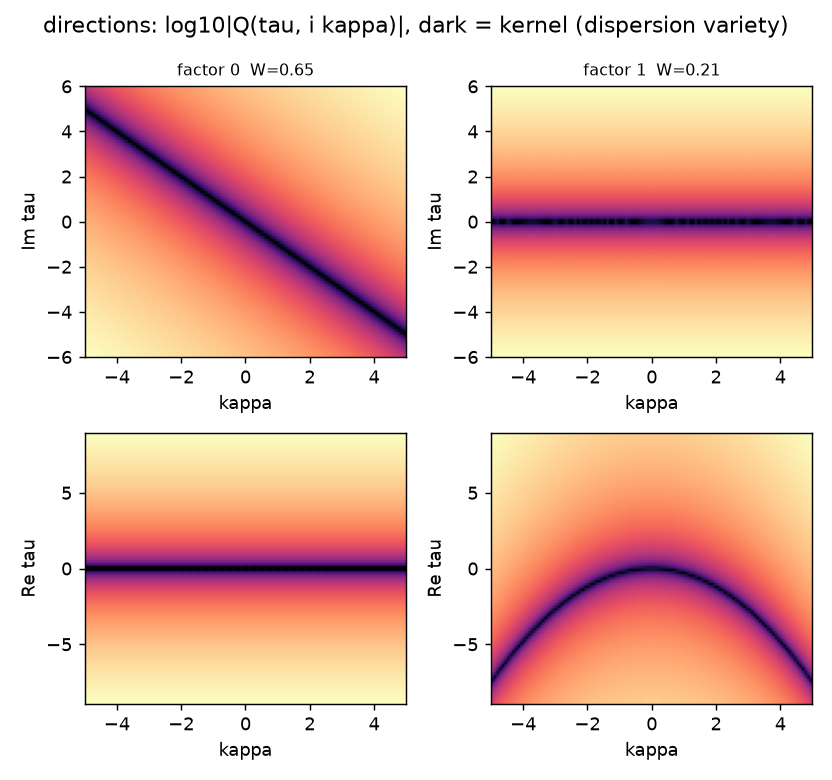
\includegraphics[width=0.8\linewidth]{sm_directions}
\caption{\texttt{directions.png}: each column is one reported factor; dark curves are the modes it can carry. Left:
transport (tilted in the oscillation row, flat in the damping row). Right: diffusion (flat in the oscillation row, a
parabola in the damping row).}\label{sm:fig:directions}
\end{figure}

\paragraph{Separation of the factors} The image \texttt{operator\_space.png} (\cref{sm:fig:opspace}) compares the reported
factors and the factors found in the posterior samples by the largest principal angle between their solution spaces. Two
compact blocks far apart mean two well separated factors on which the samples agree; a spread-out cloud, or samples
halfway between two factors, means that the samples disagree about the structure; two reported factors close together
mean a small $\gN$ and wide intervals for the components.

\begin{figure}[htbp]
\centering
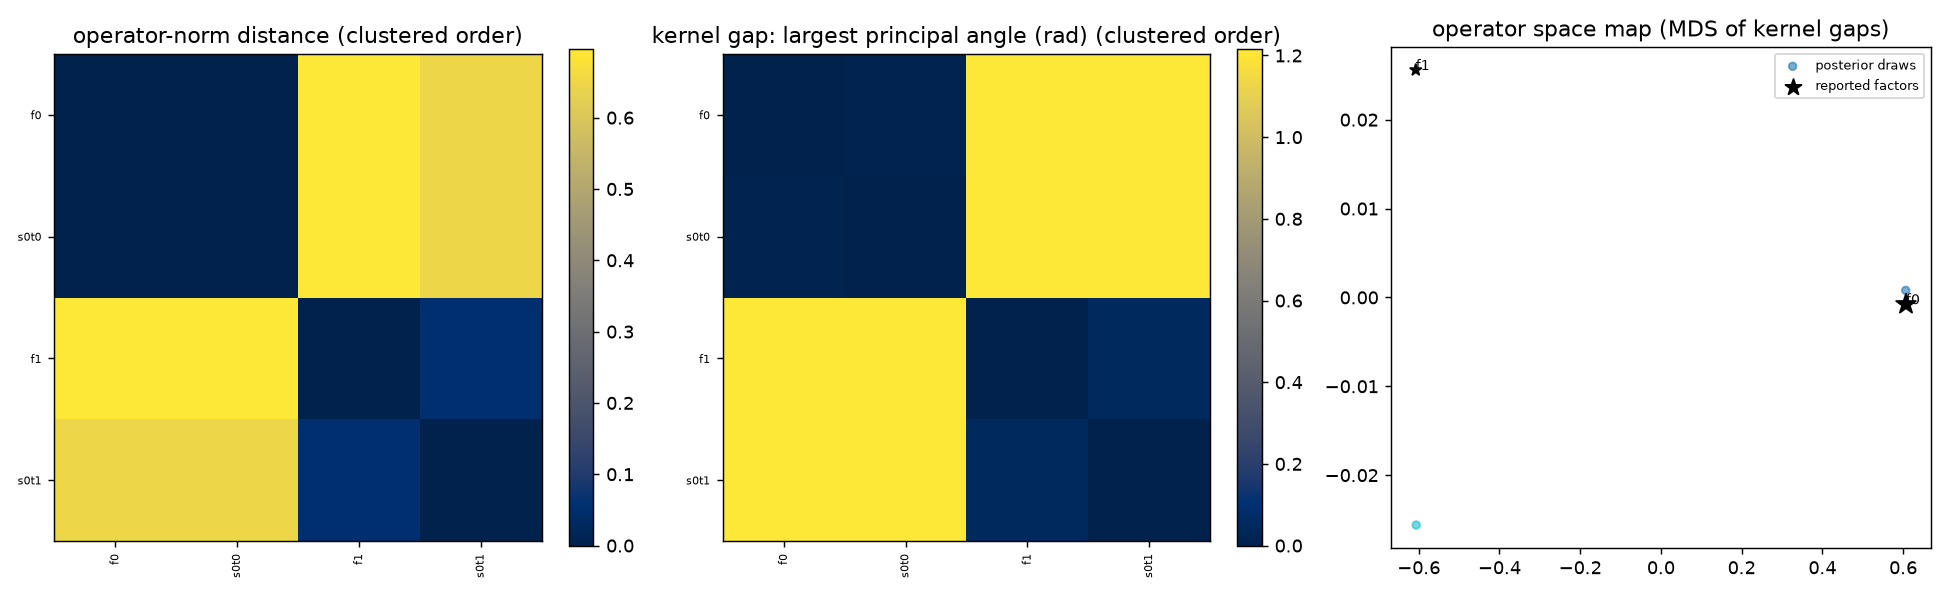
\includegraphics[width=\linewidth]{sm_operator_space}
\caption{\texttt{operator\_space.png}. Left: distance between operators. Middle: largest principal angle between the
solution spaces of every pair of factors (the reported factors \texttt{f0}, \texttt{f1} and the factors \texttt{s0t0},
\texttt{s0t1} found in the field sample), ordered by cluster; dark diagonal blocks are the groups, about $1.2$ rad apart.
Right: a two-dimensional map of these angles; stars are the reported factors, dots the factors of the
samples.}\label{sm:fig:opspace}
\end{figure}

\paragraph{Components} The image \texttt{modes\_and\_components.png} shows, for each factor, a few of its kernel modes and
the component $u_j$ of the data attributed to it; the components add up to the data up to the residual. If a component
looks like noise, or like a copy of another, that factor is not well separated. \texttt{directions\_uncertainty.png}
shows where the posterior samples disagree about each curve, and \texttt{distributions.png} the histograms of $\cF$, $\gN$
and $\rho$ over the samples.

\paragraph{Five questions to ask of any result}
\begin{enumerate}
\item What is the label? Anything other than \FC: read the note that comes with it.
\item Are the factors separated? $P(\text{split})$ close to one, $\gN$ not tiny, two distinct blocks in
\cref{sm:fig:opspace}.
\item Is each coefficient narrow and nonzero? Look at the $90\%$ interval of every term.
\item Does the model pass the tests? No $\log_{10}p$ below $-3$.
\item Do the pictures look like physics? Clean dark curves, components that look like the data, posterior samples on top
of the reported factors.
\end{enumerate}



\section{Beyond linear equations with constant coefficients}\label{sm:beyond}
The results of the paper rest on one structure: candidate equations form the commutative ring $\C[\tau,\xi]$, solutions
form vector spaces, and the exact sequence of \cref{sm:proof-factor} turns a factorization of the symbol into a splitting
of the solution. \Cref{sm:tab:beyond} summarizes what carries over when this structure is weakened; the paragraphs below
explain the three directions in one example each.

\begin{table}[htbp]
\centering\small
\caption{What carries over beyond scalar linear equations with constant coefficients.}\label{sm:tab:beyond}
\begin{tabularx}{\linewidth}{@{}>{\raggedright\arraybackslash}p{2.1cm}>{\raggedright\arraybackslash}X>{\raggedright\arraybackslash}X>{\raggedright\arraybackslash}X@{}}
\toprule
Setting & Candidate equations & Groups & What survives\\
\midrule
linear, constant coefficients & commutative ring $\C[\tau,\xi]$; unique factorization & factors of the symbol, overlap
$\deltaP$ & everything in the paper\\
higher space dimension & $\C[\tau,\xi_1,\dots,\xi_d]$ & hypersurfaces; two factors may share a whole curve & the pencil per
wavenumber vector; grouping I\\
variable coefficients & non-commutative Weyl algebra; no unique factorization & no general splitting theorem & local rates
$\lambda(\kappa;x_0)$; identification in a finite class of coefficients\\
nonlinear & a finite dictionary of jet monomials & none (no superposition) & the interaction term and its short-time
expansion\\
\bottomrule
\end{tabularx}
\end{table}

\paragraph{Higher dimension} In $d$ space dimensions the matrix pencil still reads the temporal rates at each wavenumber
vector $\kappa\in\R^d$, one small eigenvalue problem per wavenumber, and the groups become hypersurfaces
$Q_j(\lambda,i\kappa)=0$ that grouping I can fit in the same way. What is missing is the analogue of
\cref{thm:factor}: in $d+1\ge3$ variables two coprime factors can share a whole curve of zeros, and the overlap is no
longer finite-dimensional.

\paragraph{Variable coefficients} If the coefficients vary slowly in $x$, a windowed transform gives local rates
$\lambda(\kappa;x_0)$, and each group becomes a family of curves indexed by position; grouping I would then fit
coefficient functions instead of numbers. The operators now form a non-commutative algebra ($\partial_x\,x-x\,\partial_x=1$),
factorization is not unique, and with arbitrary coefficients one solution identifies nothing: any $u$ without zeros solves
$(\partial_x-u_x/u)u=0$. Identification is possible only inside a fixed finite-dimensional class of coefficients; for
$iu_t=-u_{xx}+V(x)u$, for instance, $V=(iu_t+u_{xx})/u$ wherever $u\neq0$.

\paragraph{Nonlinear equations} For $u_t=\sum_n\mathcal A_n(u)$ the definition~\eqref{sm:eq:eint} of the interaction still
makes sense, and for short times
\[
  \Eint(t)=\frac{t^2}{2}\sum_{n\neq m}\mathcal A_n'[u_0]\big(\mathcal A_m(u_0)\big)+O(t^3),
\]
with $\mathcal A_n'$ the Fr\'echet derivative: the flow is its linearization plus a quadratic interaction. For Burgers'
equation $u_t=-uu_x+\nu u_{xx}$ this gives $\Eint(t)=-\nu(u_0u_0'''+2u_0'u_0'')\,t^2+O(t^3)$, valid while the solution is
smooth. So modes of the linearized flow can still be grouped on short windows, and the size of $\Eint$ tells whether the
groups persist. Without a ring there is no analogue of $\deltaP$, of the projectors~\eqref{eq:lagrange} or of $\gN$; in
each direction the first task is therefore the one carried out in the paper for the linear case.

\section{Code and data}\label{sm:code}
The archive \texttt{code\_and\_data.zip} is a snapshot of the repository~\cite{Pri26code} at the version that produced
every number of the paper; later versions are maintained there. Its file \texttt{CONTENTS.txt} lists every file. In short:
\begin{itemize}
\item \texttt{code/pdefactor/}: the complete algorithm as a Python package (entry point \texttt{run\_loop});
\texttt{python -m pdefactor.demo} runs it on a simulated equation in under a minute.
\item \texttt{example\_run/}: the worked example of \cref{sec:worked}, run with the benchmark protocol, with the full
text report and the five images described in \cref{sm:reading}, so the output can be inspected without running anything.
\item \texttt{benchmarks/}: the scripts of both benchmarks and all their stored per-input results, among them
\texttt{out/large.jsonl} (one row per random equation, with the true factors and both methods' answers).
\item The folder \texttt{claude/\allowbreak benchmark\_tables/} holds the benchmark tables, among them \texttt{large.md} and
\texttt{p8\_final\_v5.md}, from which \cref{tab:large,tab:bench} are taken (the folder keeps its name from the
repository so that the scripts run unchanged).
\item \texttt{code/experiments/}: the experiment scripts and those that produce the figures of the paper from the
stored results; \texttt{tests/}: the test suite.
\end{itemize}
The \texttt{README.md} of the archive gives the commands to install the package, rerun the example, reproduce both
benchmarks and regenerate the figures.


\Needspace{8\baselineskip}
\begin{thebibliography}{10}

\bibitem{Bre11}
Haim Brezis.
\newblock {\em Functional Analysis, Sobolev Spaces and Partial Differential Equations}.
\newblock Universitext. Springer, New York, 2011.

\bibitem{CLO15}
David~A. Cox, John Little, and Donal O'Shea.
\newblock {\em Ideals, Varieties, and Algorithms}.
\newblock Undergraduate Texts in Mathematics. Springer, Cham, 4 edition, 2015.

\bibitem{Deu01}
Frank Deutsch.
\newblock {\em Best Approximation in Inner Product Spaces}.
\newblock CMS Books in Mathematics. Springer, New York, 2001.

\bibitem{Ful08}
William Fulton.
\newblock {\em Algebraic Curves: An Introduction to Algebraic Geometry}.
\newblock 2008.
\newblock Electronic edition of the 1969 book (W.\,A. Benjamin, New York).

\bibitem{Gau62}
Walter Gautschi.
\newblock On inverses of {V}andermonde and confluent {V}andermonde matrices.
\newblock {\em Numerische Mathematik}, 4:117--123, 1962.

\bibitem{Pri26code}
Flavio Pricoco.
\newblock pde-factor-fit: reading the factor structure of linear {PDE}s from data.
\newblock \url{https://github.com/FlavioApric/pde-factor-fit}, 2026.
\newblock Software and benchmark data.

\bibitem{Rha55}
Georges de~Rham.
\newblock {\em Vari\'et\'es diff\'erentiables: formes, courants, formes harmoniques}.
\newblock Hermann, Paris, 1955.

\end{thebibliography}

\end{document}
